% !TEX program = pdflatex
\documentclass[11pt,a4paper]{article}

\usepackage[utf8]{inputenc}
\usepackage[T1]{fontenc}
\usepackage{lmodern}
\usepackage{geometry}
\geometry{margin=1in}
\usepackage{amsmath,amssymb}
\usepackage{siunitx}
\usepackage{graphicx}
\usepackage[font=small,labelfont=bf,labelsep=endash]{caption}
\usepackage{booktabs}
\usepackage{physics}
\usepackage{cite}
\usepackage{hyperref}
\usepackage{float}
\hypersetup{colorlinks=true,linkcolor=blue,citecolor=blue,urlcolor=blue}

\title{Design Methodology for a Dual-Jet Hovering Disc with Concentric Air Curtains:\\
Model, Non-Dimensionalization, and Physical Assumptions}
\author{ }
\date{ }

\begin{document}

\maketitle

\begin{abstract}
This paper presents a design-oriented physical model for a hovering disc sustained by two concentric air jets:
an outer annular jet that forms an aerodynamic curtain to confine the inner flow and an inner jet that maintains the central cushion pressure.
The analysis uses a low-Mach compressible, axisymmetric core model with an anisotropic Stokes--Darcy closure to approximate the pressure and velocity fields in the cushion region.
A detailed discussion of the model's assumptions and their physical validity is provided, along with a complete nomenclature of symbols used throughout the work.
\end{abstract}

\begin{figure}[t]
  \centering
  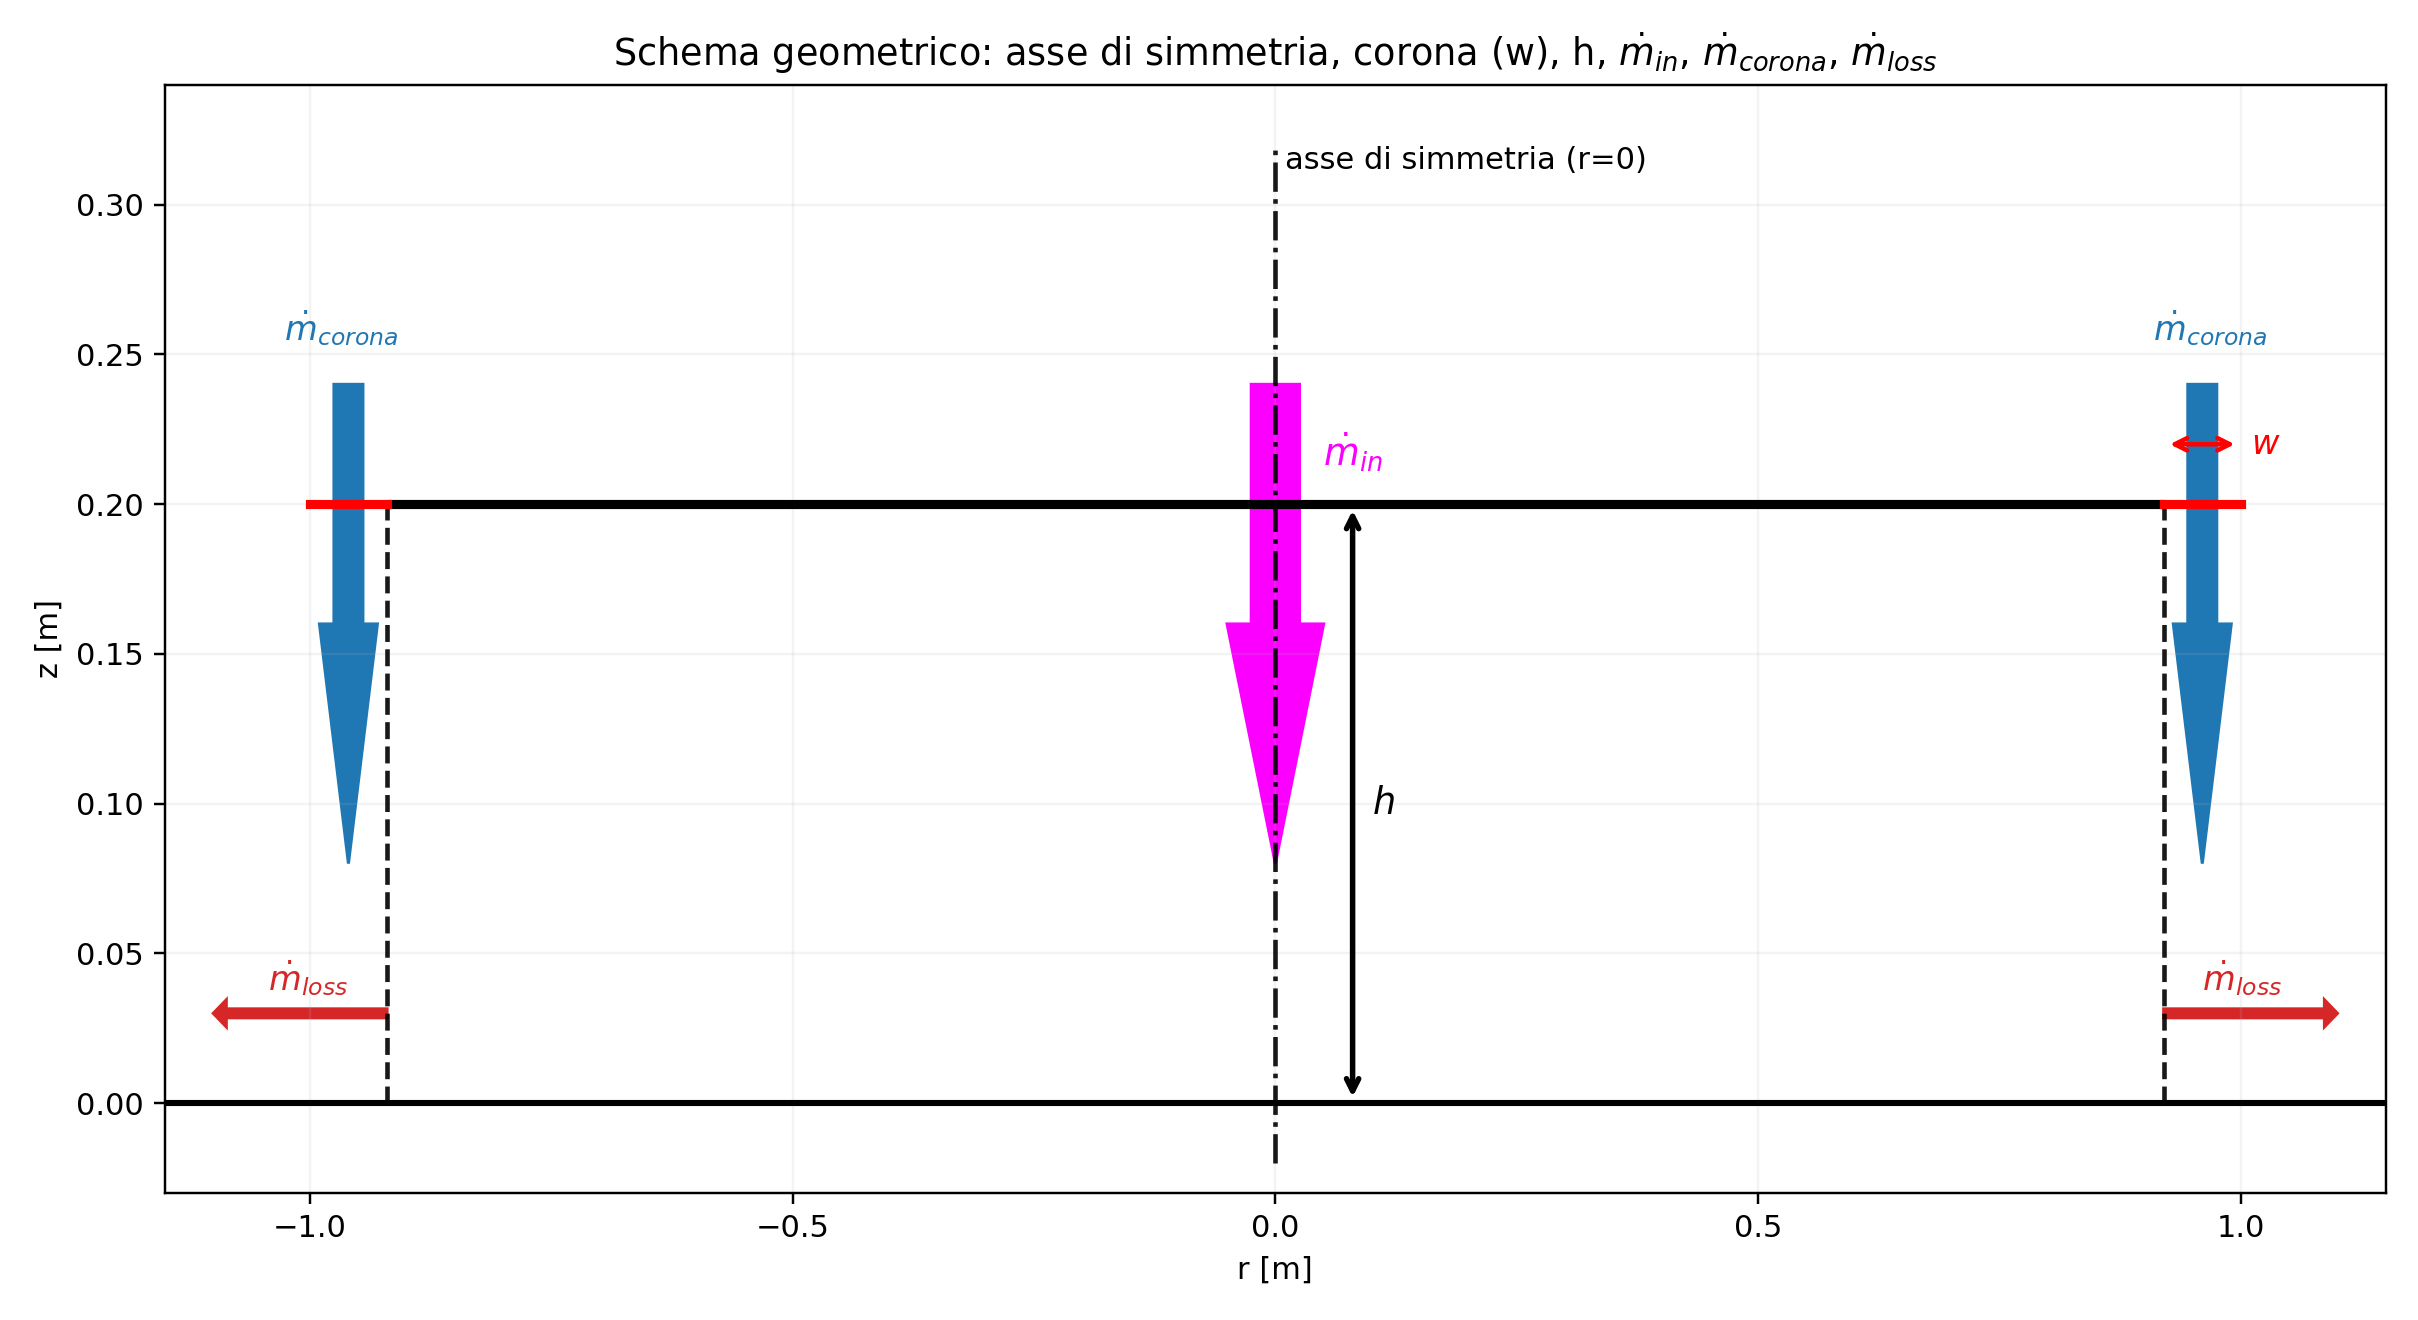
\includegraphics[width=0.95\linewidth]{../figs/schema_geometry.png}
  \caption{Schematic of the hovering disc with two concentric jets: the outer annular curtain and the central make-up flow.}
  \label{fig:geometry}
\end{figure}\begin{figure}[H]
  \centering
  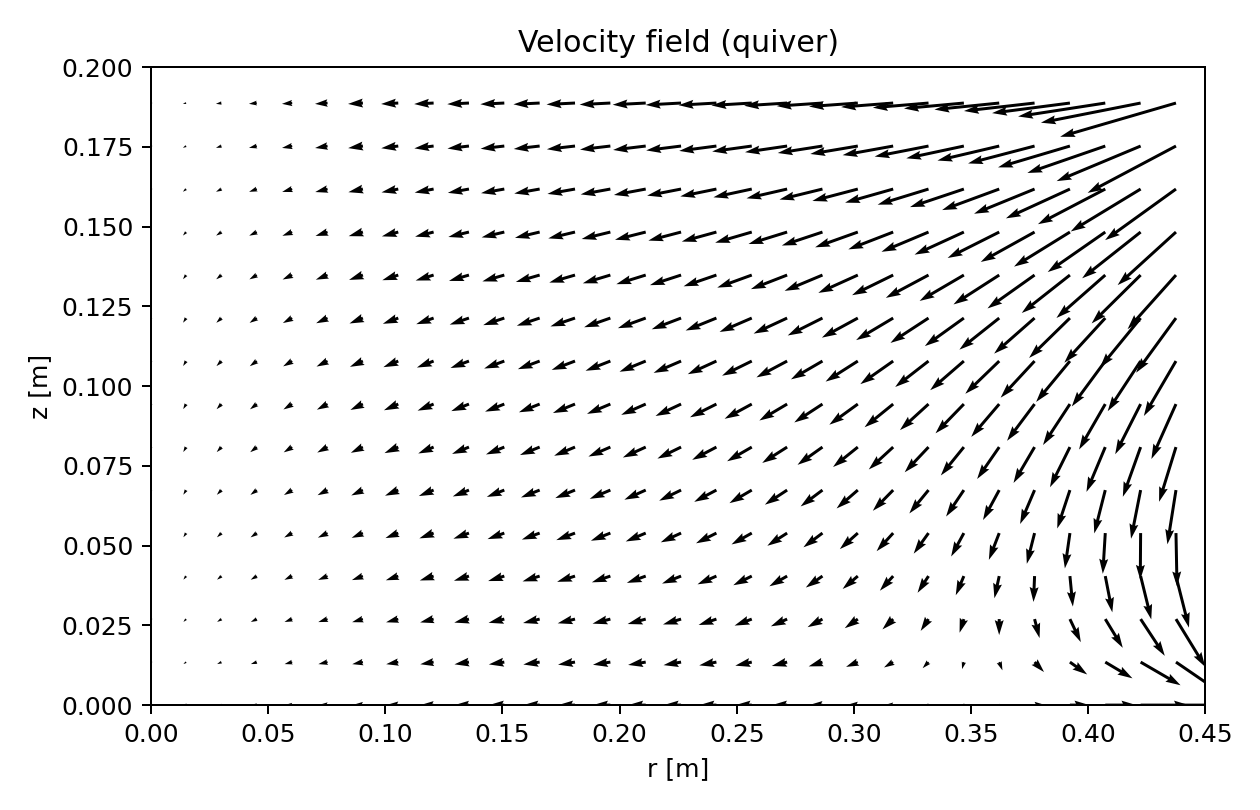
\includegraphics[width=0.95\linewidth]{../figs/quiver_velocity.png}
  \caption{Non-dimensional velocity field (quiver).
Vectors show $(\hat u,\,S\hat w)$ for isotropic visual scaling; the pattern reflects the rim-imposed sealing pressure from the downward curtain.}
  \label{fig:quiver}
\end{figure}\begin{figure}[H]
  \centering
  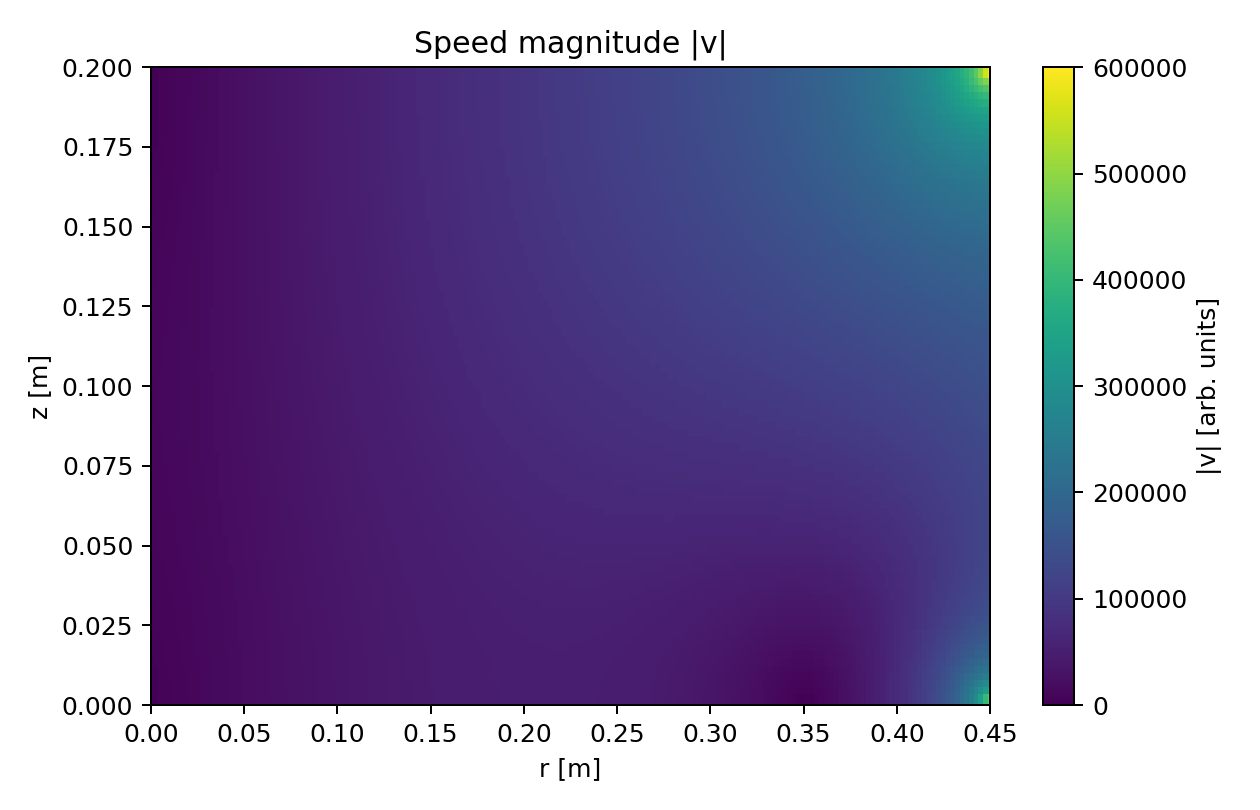
\includegraphics[width=0.95\linewidth]{../figs/cmap_speed.png}
  \caption{Colormap of the non-dimensional isotropic speed magnitude $\hat V_{\mathrm{iso}}=\sqrt{\hat u^{\,2}+S^{2}\hat w^{\,2}}$.}
  \label{fig:cmap_speed}
\end{figure}\begin{figure}[H]
  \centering
  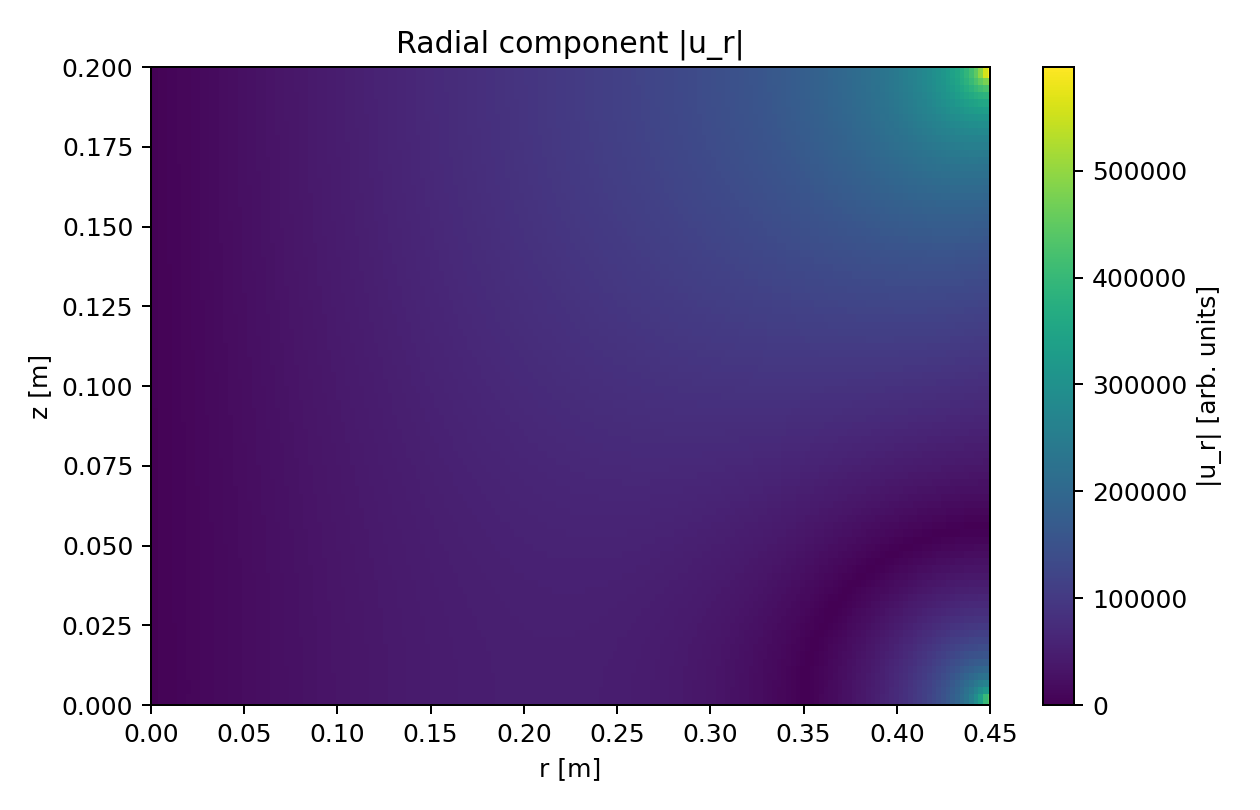
\includegraphics[width=0.95\linewidth]{../figs/cmap_ur.png}
  \caption{Colormap of the non-dimensional radial component magnitude $|\hat u|$.}
  \label{fig:cmap_ur}
\end{figure}\begin{figure}[H]
  \centering
  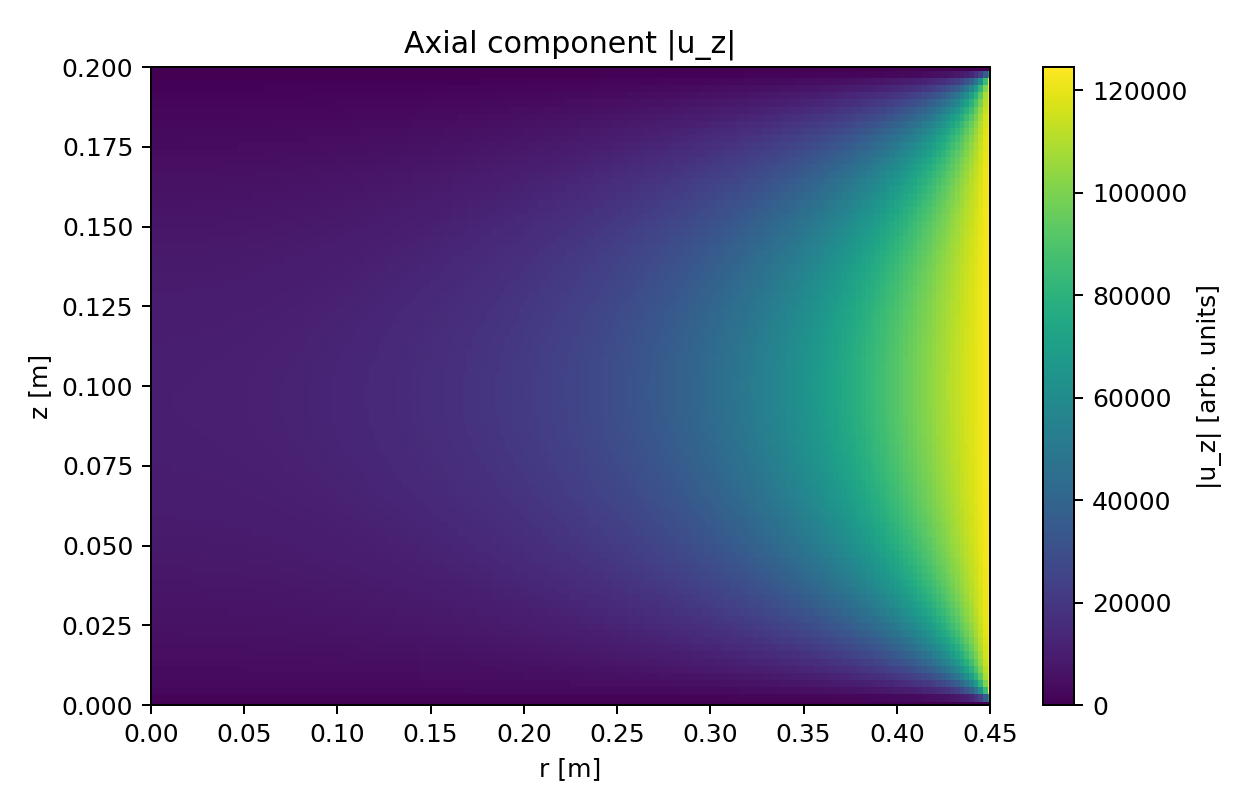
\includegraphics[width=0.95\linewidth]{../figs/cmap_uz.png}
  \caption{Colormap of the non-dimensional axial component magnitude $|\hat w|$.}
  \label{fig:cmap_uz}
\end{figure}\begin{figure}[H]
  \centering
  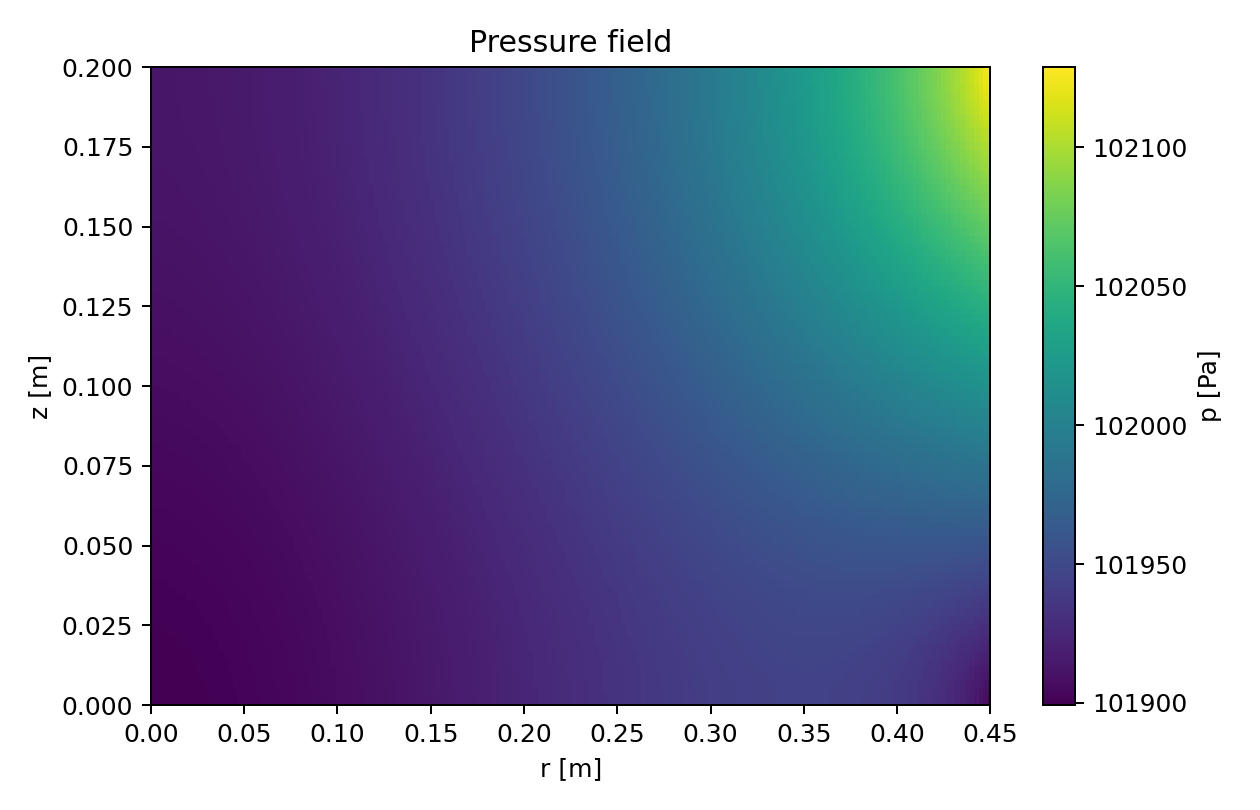
\includegraphics[width=0.95\linewidth]{../figs/cmap_pressure.png}
  \caption{Colormap of the non-dimensional pressure $\hat p$.}
  \label{fig:cmap_p}
\end{figure}\section{Geometry and Notation}
\label{sec:geometry}
The geometry follows Fig.~\ref{fig:geometry}, defining the coordinate system and characteristic dimensions:
\begin{itemize}
  \item $R_{\mathrm{tot}}$ -- total radius of the disc.
  \item $h$ -- hovering height from the ground.
  \item $w$ -- width of the peripheral leakage ring; $R^{-}=R_{\mathrm{tot}}-w$ is its inner radius.
  \item $b$ -- thickness of the outer annular jet slot.
  \item $h_{\mathrm{eff}}$ -- effective sealing height (characteristic of curtain recirculation).
  \item $p_0$ -- ambient pressure; $p_c=W/(\pi R_{\mathrm{tot}}^2)$ -- cushion pressure supporting the load $W$.
  \item $U_{\mathrm{out}}$, $\rho_j$ -- speed and density of the outer jet.
  \item $\mu$ -- dynamic viscosity; $R_g$ -- specific gas constant for air.
  \item $\dot{m}_{\mathrm{in}}$ -- air mass flow entering internal region.
  \item $\dot{m}_{\mathrm{out}}$ -- air mass flow of outer region.
  \item $\dot{m}_{\mathrm{loss}}$ -- air mass flow exiting internal region.
  \item $b_0$ -- slot thickness of the outer curtain jet at injection.
  \item $H$ -- effective curtain height (equal to $h$ in this study, representing the vertical extent over which the curtain resists leakage).
\end{itemize}

\section{Model Overview}
\label{sec:model-overview}

The cushion region ($0\le r\le R^{-},\ 0\le z\le h$) is filled with air at variable pressure, temperature, and density.
The mean flow satisfies an anisotropic Stokes--Darcy closure:
\begin{equation}
  u = -\frac{\kappa_r}{\mu}\,\partial_r p,\qquad
  w = -\frac{\kappa_z}{\mu}\,\partial_z p,
\end{equation}
with permeability coefficients $\kappa_r=\alpha_r h^2$ and $\kappa_z=\alpha_z h^2$, where $\alpha_r$ and $\alpha_z$ are empirical dimensionless parameters encoding the overall resistance of the confined air layer.

The continuity and state relations read
\begin{equation}
  \frac{1}{r}\,\partial_r\!\left(r\rho u\right)+\partial_z(\rho w)=0,\qquad
  p=\rho R_g T.
\end{equation}
Elimination of $u,w$ gives the pressure formulation:
\begin{equation}
  \frac{1}{r}\partial_r(r\rho\kappa_r\partial_r p)+\partial_z(\rho\kappa_z\partial_z p)=0.
\end{equation}




\section{Simulation Methodology}
\label{sec:simulation-method}

This section provides the complete, deterministic simulation procedure used to size the system and to predict how the air behaves in each part of the domain. The approach enforces \emph{stationarity} both in the pressurized \emph{core (cushion)} and in the \emph{outer jet/wall-jet} that seals the cushion along the ground. At stationarity, the pressure field in the core and the momentum/thickness fields in the wall-jet are coupled by mass and momentum balances and by a pressure-jump condition at the rim.

\subsection{Objectives}
Given the geometry $(R_{\mathrm{tot}},\, h,\, b,\, w)$ and the target core overpressure $\Delta p=p_c-p_0$, the simulation determines the injection speeds of the inner/core and outer jets, $U_{\mathrm{core}}$ and $U_{\mathrm{out}}$, and the radial distributions of the sealing wall-jet, namely its characteristic speed $U_c(r)$ and thickness $\delta(r)$. From these, we evaluate: (i) the pressure needed to sustain the cushion; (ii) how the $\Delta p$ between core and ambient biases the outer jet; (iii) to what extent the outer jet can maintain the high core pressure thanks to its high speed and to the presence of the ground beneath the disc; and (iv) global performance metrics (leakage, power, sealing efficiency).

\subsection{Core (cushion) equilibrium and velocity profile}
Inside the cushion ($0\le r\le R^{-},\ 0\le z\le h$) we adopt the anisotropic Stokes--Darcy closure
\begin{equation}
  u = -\frac{\kappa_r}{\mu}\,\partial_r p,\qquad
  w = -\frac{\kappa_z}{\mu}\,\partial_z p,\qquad 
  \kappa_r=\alpha_r h^2,\;\kappa_z=\alpha_z h^2,
\end{equation}
with continuity and ideal-gas state
\begin{equation}
  \frac{1}{r}\,\partial_r\!\left(r\rho u\right)+\partial_z(\rho w)=0,\qquad
  p=\rho R_g T .
\end{equation}
At stationarity the core pressure $p(r,z)$ solves
\begin{equation}
  \partial_r\!\left(r\rho\kappa_r\partial_r p\right)+r\,\partial_z\!\left(\rho\kappa_z\partial_z p\right)=0.
\end{equation}
The core is driven by an inner vertical jet of speed $U_{\mathrm{core}}$ and area $A_{\mathrm{core}}$; its flow rate is adjusted so that the areal-mean core pressure matches the design value $p_c=p_0+\Delta p$ while satisfying the sealing condition at the rim (Sec.~\ref{sec:coupling}). The depth-averaged core velocity profile is then
\begin{equation}
  \bar u(r) = -\frac{\kappa_r}{\mu}\,\partial_r \bar p(r),\qquad 
  \bar p(r)=\frac1h\int_0^h p(r,z)\,dz ,
\end{equation}
which we use to compute the radial mass flux exiting the cushion across the seal strip.

\subsection{Outer annular jet and wall-jet equilibrium}
The outer annular jet of thickness $b$ is injected downward at the rim with speed $U_{\mathrm{out}}$. After impingement at radius $r_t$ it turns into a ground-attached wall-jet that flows inward over the floor toward $r_-$, providing dynamic sealing. Its self-similar velocity profile is represented as
\begin{equation}
  u(r,z) = U_c(r)\, f\!\left(\eta\right),\qquad \eta=\frac{z}{\delta(r)} ,
\end{equation}
where $U_c(r)$ and $\delta(r)$ are obtained from integral balances. The wall-jet thickness grows as
\begin{equation}
  \frac{d\delta}{dr} = k_e - E\,\frac{\delta}{q}\,\left(p(r,0)-p_0\right),
\end{equation}
while the mass and streamwise momentum per unit circumference, $q(r)$ and $m(r)$, satisfy
\begin{align}
  \frac{dq}{dr} &= E\,\rho_\infty U_c(r) - \underbrace{\frac{1}{R_g T_\infty}\,\delta(r)\,\frac{dp}{dr}}_{\text{baroclinic work}},\\
  \frac{dm}{dr} &= -C_f\,\rho_\infty \frac{U_c^2(r)}{\delta(r)} - K_{\mathrm{turn}}\,\delta(r_t)\,U_c^2(r_t)\,\delta(r-r_t) ,
\end{align}
with $C_f=C_{f0}\,Re_\delta^{-1/5}$ and $Re_\delta=\rho_\infty U_c\delta/\mu$. The constitutive profile gives $q=\rho_\infty U_c\delta I_1$ and $m=\rho_\infty U_c^2\delta I_2$, where $I_1,I_2$ are shape factors of $f(\eta)$ (constants once the profile family is chosen).

\subsection{Coupling via rim pressure-jump and mass closure}\label{sec:coupling}
Stationarity imposes two conditions at the sealing strip $[r_-,R^{-}]$:
\begin{enumerate}
  \item \textbf{Pressure jump:} the inner core pressure exceeds ambient by $\Delta p$ and is supported by the wall-jet momentum flux plus losses across the strip,
  \begin{equation}
    \Delta p = \frac{m(r_-)}{\delta_p} + \Lambda_{\mathrm{loss}} ,
  \end{equation}
  where $\delta_p$ is the effective thickness for pressure work and $\Lambda_{\mathrm{loss}}$ collects minor-loss contributions.
  \item \textbf{Mass balance:} the net radial mass efflux from the core equals the wall-jet inflow delivered by the outer annular jet after turning and entrainment,
  \begin{equation}
    2\pi\!\int_0^{R^{-}}\!\rho \bar u(r)\,h\,dr \;=\; 2\pi r_t\,\rho_j U_{\mathrm{out}} b\;+\;\int_{r_-}^{r_t}\! E\,\rho_\infty U_c(r)\,dr .
  \end{equation}
\end{enumerate}
These two conditions, together with the wall-jet integral equations, determine $U_{\mathrm{core}}$, $U_{\mathrm{out}}$, and the profiles $U_c(r)$ and $\delta(r)$.

\subsection{Deterministic solution algorithm}
The unknowns are $U_{\mathrm{core}}$, $U_{\mathrm{out}}$, and the fields $\{U_c(r),\delta(r)\}$. The algorithm is as follows:
\begin{enumerate}
  \item \textbf{Core solve.} For a trial $U_{\mathrm{core}}$, solve the core pressure problem to obtain $\bar p(r)$ and the core outflow across the seal strip.
  \item \textbf{Wall-jet integration.} For a trial $U_{\mathrm{out}}$, initialize at $r=r_t$ with $(\delta_t, U_c(r_t))$ set by slot kinematics and turning loss $K_{\mathrm{turn}}$, then integrate the mass--momentum ODEs for $\{q(r),m(r)\}$ inward to $r_-$; recover $U_c(r)$ and $\delta(r)$ from the chosen profile shape.
  \item \textbf{Coupling.} Evaluate the pressure-jump residual and the mass residual at the rim; update $(U_{\mathrm{core}},U_{\mathrm{out}})$ with a 2D Newton or safeguarded secant step.
  \item \textbf{Convergence.} Iterate until both residuals fall below tolerance; then compute leakage, sealing efficiency, and power.
\end{enumerate}

\subsection{Sizing and parametric exploration}
To size the system, we sweep $(h,b,\Delta p)$ (and, if needed, $E,C_f,K_{\mathrm{turn}}$) and record the converged $(U_{\mathrm{core}},U_{\mathrm{out}})$, leakage rate, and power. This reveals how the pressure difference biases the outer jet and how the outer jet, aided by the ground, sustains the high core pressure.


\section{Validity of Modeling Assumptions}
\label{sec:validity-of-modeling-assumptions}

\subsection{Low-Mach Compressibility}
The jets have typical velocities $U_{\mathrm{out}}\approx30$--$60\,$m/s, leading to a Mach number $Ma=U/a\approx0.1$--$0.2$ with $a\simeq343\,$m/s.
This regime justifies a \emph{low-Mach} formulation: the flow is compressible enough to exhibit pressure- and temperature-dependent density, but acoustic effects remain negligible.
Hence, the ideal-gas relation $p=\rho R_g T$ is retained, while the flow is assumed quasi-static in time.

\subsection{Thermal Uniformity and Energy Exchange}
Although the confined air experiences some compression heating, the characteristic time scales of thermal diffusion and convective mixing by the curtain are short compared to global unsteadiness.
The first-order model therefore assumes a uniform temperature $T=T_\infty$, with the understanding that future extensions may include the steady energy balance to recover small deviations of $T(r,z)$.

\subsection{Stokes--Darcy Closure}
The Stokes--Darcy model does not imply a porous medium in the literal sense.
Instead, it approximates the momentum balance of a low-Reynolds, highly dissipative, confined flow.
At low $Re=\rho U h/\mu$, the Stokes equations reduce to a linear proportionality between pressure gradient and velocity.
Replacing $\nabla^2\mathbf{u}\sim \mathbf{u}/L^2$ with an effective geometric length $L\sim h$ yields
\begin{equation}
  \mathbf{u}\approx-\frac{h^2}{\mu}\nabla p,
\end{equation}
which is mathematically equivalent to Darcy's law with an effective permeability $\kappa\sim h^2$.
The anisotropic form used here,
\begin{equation}
  \kappa_r=\alpha_r h^2,\qquad \kappa_z=\alpha_z h^2,
\end{equation}
accounts for different confinement levels in the radial and vertical directions.

\paragraph{Validity range.}
This closure is valid provided that:
\begin{itemize}
  \item the Reynolds number in the cushion $Re_c=\rho U_c h/\mu \ll 1$;
  \item pressure variations are slow and inertia negligible;
  \item the flow is quasi-steady and dominated by viscous losses and boundary friction;
  \item local turbulence and recirculation effects are absorbed into the empirical coefficients $\alpha_r,\alpha_z$.
\end{itemize}
It is particularly suited to parametric design and control studies where the detailed jet micro-structure is not resolved.

\subsection{Boundary Conditions and Curtain Coupling} \label{sec:boundaryconditions}
The outer slot jet issues \emph{downwards} and acts as an \emph{air curtain} that
limits radial leakage from the cushion. The pressure imposed along the rim
$r=R^{-}$ is modeled as the superposition of two physically motivated
contributions:
\begin{equation}
  p_{\mathrm{edge}}(z)=p_0 + \min\!\Big(\Delta P,\;\frac{\rho\,U(z)^2\,b(z)}{H\,D_{m,\min}}\Big),\qquad \zeta=\frac{z}{H}.
  \label{eq:p_edge_momentum}
\end{equation}

On $z=0$ and $z=h$ we impose no-normal-flow in the reduced core model
\begin{equation}
  \partial_z p(r,0)=\partial_z p(r,h)=0,
\end{equation}
while $r=0$ enforces symmetry $\partial_r p(0,z)=0$. The inner make-up jet is not
imposed as a local BC in the core; its effect enters the \emph{global} mass balance
(see Sec.~\ref{sec:simulation-method}).
This expression guarantees continuity of rim pressure along $z$ and smoothly connects
the low static pressure region at the slot exit with the higher static build-up near the
floor.

\paragraph{Remark on sealing vs static pressure.}
The composite rim pressure in Eq.~\eqref{eq:p_edge_momentum} is a
\emph{modeling device}: the $(1-\zeta)^n$ term provides a minimal representation
of static-pressure build-up as the curtain turns near the floor, while the
$\zeta^m$ term encodes the sealing effectiveness of a high-momentum jet near the slot.
This separation avoids conflating the jet's low static pressure near the slot with
its strong \emph{barrier} effect on radial leakage.

\section{Non-Dimensionalization and Plotting Conventions}
\label{sec:non-dimensionalization-and-plotting-conventions}

We scale
\begin{equation}
  \hat r=\frac{r}{R_{\mathrm{tot}}},\quad
  \hat z=\frac{z}{h},\quad
  \hat p=\frac{p-p_0}{p_c},\quad
  \hat T=\frac{T}{T_\infty},\quad
  \hat\rho=\frac{\rho}{\rho_\infty}
  =\frac{1+\Pi_p\,\hat p}{\hat T},\qquad
  \Pi_p=\frac{p_c}{p_0}.
\end{equation}
with boundary conditions
\begin{equation}
  \partial_{\hat r}\hat p(0,\hat z)=0, \qquad
  \partial_{\hat z}\hat p(\hat r,0)=\partial_{\hat z}\hat p(\hat r,1)=0, \qquad
  \hat p(\hat R^{-},\hat z)=\hat p_{\mathrm{edge}}(\hat z),
\end{equation}
where
\begin{equation}
  \hat p_{\mathrm{edge}}(\hat z)
  =\frac{1}{p_c}\,
   \min\!\Big(
      \Delta P,\;
      \frac{\rho\,U(z)^2\,b(z)}{H\,D_{m,\min}}
    \Big),
  \qquad
  \hat z=\frac{z}{H}.
\end{equation}
Here $\hat R^{-}=R^{-}/R_{\mathrm{tot}}$, and in this study we set $H=h$
for consistency with the gap height.  The pressure distribution
$\hat p_{\mathrm{edge}}(\hat z)$ represents the momentum-based
sealing effect of the air curtain according to
Eq.~\eqref{eq:p_edge_momentum}.

Natural velocity scales are
\begin{equation}
  U_r^0=\frac{\kappa_r}{\mu}\,\frac{p_c}{R_{\mathrm{tot}}},\qquad
  U_z^0=\frac{\kappa_z}{\mu}\,\frac{p_c}{h},\qquad
  S=\frac{U_z^0}{U_r^0}
  =\frac{\alpha_z}{\alpha_r}\,\frac{R_{\mathrm{tot}}}{h}.
\end{equation}
The dimensionless velocities used for plotting are
\begin{equation}
  \hat u=-\partial_{\hat r}\hat p,\qquad
  \hat w=-\partial_{\hat z}\hat p,\qquad
  \hat V_{\mathrm{iso}}=\sqrt{\hat u^{\,2}+S^{2}\hat w^{\,2}}.
\end{equation}

\section{Simulation Outputs}
\label{sec:simulation-outputs}

The results produced from the model are shown in this section.
\section{Model Limitations and Planned Extensions}
\label{sec:model-limitations-and-planned-extensions}

The Darcy--Brinkman closure is an engineering reduction (effective permeability in a
free flow); $\alpha_r,\alpha_z$ should be calibrated against axisymmetric CFD.
The make-up jet is not imposed as a local BC in the core; it enters only via the
mass-balance closure. Thermal effects are neglected ($T=T_\infty$). The bypass parameter
$\beta$ is defined conceptually but not used yet in the code; it will be included together
with the automated shooting loop and power estimates.

\paragraph{Appendix: minimal rationale for the composite rim pressure.}
Consider a control volume hugging the rim over height $h$ and thickness $O(b)$.
A downward slot jet of density $\rho_j$ and speed $U_{\mathrm{out}}$ is deflected
into a radial wall-jet of speed $U_r(z)$ near the floor. A crude momentum balance
suggests a static build-up $\Delta p_{\mathrm{stat}}\sim \rho_j U_{\mathrm{out}}^2
\,\mathcal{O}(1)$ concentrated near $\zeta\!\to\!0$, while the resistance to
cross-flow (sealing) scales with the jet momentum flux impinging near the slot,
$\Delta p_{\mathrm{seal}}\sim \rho_j U_{\mathrm{out}}^2\,\mathcal{O}(1)$ for
$\zeta\!\to\!1$. The composite form
$\rho_j U_{\mathrm{out}}^2\,[\,C_p(1-\zeta)^n + C_s \zeta^m\,]$ is thus a
first-order surrogate capturing both effects with two tunable, dimensionless
coefficients $(C_p,C_s)$ and mild shape exponents $(m,n)$.

\paragraph{On the choice of $D_{m,\min}$.}
We take $D_{m,\min}$ from air-curtain literature (order $10^{-1}$) as a design parameter; in absence of calibration, $D_{m,\min}=0.2$ provides a conservative default.
Sensitivity to this parameter is reported without altering the solver or figures.

\paragraph{On the choice of $D_{m,\min}$.}
We adopt $D_{m,\min}=0.2$ as conservative default, consistent with air-curtain literature (typical range $0.1$--$0.3$). The parameter may be refined by CFD or experimental calibration.

% =====================================================
% --- Outer Jet Impingement–Wall-Jet–Seal Equilibrium Model ---

\subsection*{Outer-Jet Impingement, Wall-Jet Transition, and Seal Equilibrium}

The outer annular jet, injected vertically downward in the ring $(r_- , R_{\mathrm{tot}})$,
impinges on the ground and is deflected radially outward due to the overpressure
$\Delta p = p_{\mathrm{core}} - p_\infty > 0$.
The geometry and $p_{\mathrm{core}}$ are fixed; the only free variables are the core and outer jet velocities,
$U_{\mathrm{core}}$ and $U_{\mathrm{out}}$.

\paragraph{Turning and wall-jet formation.}
The outer jet is treated as a vertical annular sheet that turns into a radial wall jet at
an effective radius $r_t \in [r_-, R_{\mathrm{tot}}]$.
A representative value is the centroid of the annulus,
$r_t = \tfrac12 (r_- + R_{\mathrm{tot}})$.
All the mass flow rate of the outer jet is collected at $r_t$
and redirected radially with a turning loss $K_{\mathrm{turn}} \in [0.1,0.3]$:
\begin{align}
\dot m_{\mathrm{out}} &= \rho A_{\mathrm{slot}} U_{\mathrm{out}},\\
q_t &= \frac{\dot m_{\mathrm{out}}}{2\pi r_t}, \qquad
m_t = (1-K_{\mathrm{turn}})\frac{\dot m_{\mathrm{out}} U_{\mathrm{out}}}{2\pi r_t}.
\end{align}
The near-wall jet thickness at this location is
\begin{equation}
\delta_t = \kappa_\delta b, \qquad \kappa_\delta \in [1,3].
\end{equation}

The self-similar wall-jet profile in $z$ reads
\begin{equation}
u(r,z) = U_c(r) f(\eta), \qquad \eta = z/\delta(r), \qquad
f(\eta) = \max(0, 1-\tfrac32 \eta^2 - \tfrac12 \eta^3),
\end{equation}
with shape constants
\begin{equation}
c_1 = \int_0^1 f\,d\eta, \qquad c_2 = \int_0^1 f^2\,d\eta.
\end{equation}
Local mass and momentum per unit circumference are then
$q = \rho U_c \delta c_1$ and $m = \rho U_c^2 \delta c_2$.

Momentum compatibility at the turning gives
\begin{equation}
m_t = \rho U_{c,t}^2 \delta_t c_2 =
(1-K_{\mathrm{turn}})\frac{\dot m_{\mathrm{out}} U_{\mathrm{out}}}{2\pi r_t},
\end{equation}
which provides $U_{c,t}$ and hence $q_t = \rho U_{c,t} \delta_t c_1$.
If mass and momentum do not match, $\delta_t$ is iteratively corrected keeping $K_{\mathrm{turn}}$ fixed.

\paragraph{Wall-jet evolution.}
For $r \in [r_t, R_{\mathrm{tot}}]$, the curtain evolves as a radial wall jet with entrainment
and wall friction but negligible imposed pressure gradient. The integral equations are
\begin{align}
\frac{dq}{dr} + \frac{q}{r} &= \rho E U_c, \label{eq:massbalance}\\
\frac{dm}{dr} + \frac{m}{r} &= -\tau_w, \qquad
\tau_w = \tfrac12 \rho C_f U_c^2, \qquad C_f = C_{f0} Re_\delta^{-1/5}, \label{eq:mombalance}\\
\frac{d\delta}{dr} &= k_e, \qquad \delta(r) = \delta_t + k_e (r - r_t). \label{eq:deltagrowth}
\end{align}
Closure relations: $U_c = q / (\rho \delta c_1)$, $m = \rho q^2 c_2 / (\delta c_1^2)$.

\paragraph{Seal zone and pressure equilibrium.}
In the inner strip $[r_-,\, r_- + w_s]$, with $w_s = \lambda \delta_s$,
the curtain resists the core overpressure $\Delta p$.
An integral momentum balance over this control volume gives
\begin{equation}
2\pi r_- m(r_-+w_s)
= -\!\!\int_{r_-}^{r_-+w_s} 2\pi r\,\tau_w\,dr
+ 2\pi r_- \delta_p \Delta p,
\label{eq:sealbalance}
\end{equation}
where $m(r_-)\!\approx\!0$ (no inward flow) and $\delta_p\simeq\tfrac12\delta_s$.
Equation~\eqref{eq:sealbalance} provides the required momentum flux $m(r_-+w_s)$
that the curtain must carry to balance pressure and wall losses.

Integrating Eqs.~\eqref{eq:massbalance}--\eqref{eq:deltagrowth} from $r_t$ down to $r_-+w_s$
yields $m^{(\mathrm{ODE})}(r_-+w_s; U_{\mathrm{out}})$,
which must satisfy the closure condition
\begin{equation}
m^{(\mathrm{ODE})}(r_-+w_s; U_{\mathrm{out}})
= m^{(\mathrm{seal})}(r_-+w_s; \Delta p).
\label{eq:sealeq}
\end{equation}
This nonlinear equation defines the equilibrium outer-jet velocity $U_{\mathrm{out}}$
for a given $\Delta p$ and geometry.

A first-order estimate can be expressed as
\begin{equation}
\Delta p \approx C_{\mathrm{eff}} \frac12 \rho U_c^2(r_-+w_s),
\qquad
C_{\mathrm{eff}} = \frac{c_2}{c_1^2}\frac{\delta(r_-+w_s)}{\delta_p} + \text{friction corrections.}
\end{equation}

\paragraph{Numerical procedure.}
At each iteration of the solver:
\begin{enumerate}
  \item Compute $U_{\mathrm{core}}$ from the core relation
  $p_{\mathrm{core}} = F_{\mathrm{core}}(U_{\mathrm{core}})$.
  \item Initialize the outer curtain at $r_t$ with $(\delta_t, U_{c,t})$.
  \item Integrate the wall-jet ODEs inward to obtain $m(r_-+w_s)$.
  \item Evaluate Eq.~\eqref{eq:sealbalance} and solve Eq.~\eqref{eq:sealeq} for $U_{\mathrm{out}}$.
\end{enumerate}
Typical default parameters: $K_{\mathrm{turn}}=0.2$, $\kappa_\delta=2$,
$E=0.08$, $C_{f0}=0.006$, $k_e=0.08$, $\lambda=3$, $\delta_p=0.5\delta_s$.

Physically, this closure enforces a stationary outer jet that seals the cushion
at the prescribed core pressure, ensuring negligible radial leakage.
% =====================================================
\section{Nomenclature}
\label{sec:nomenclature}

\begin{tabular}{@{}ll@{}}
\toprule
Symbol & Description \\ \midrule
$R_{\mathrm{tot}}$ & Total radius of the disc \\
$R^{-}$ & Inner radius of the leakage ring ($R^{-}=R_{\mathrm{tot}}-w$) \\
$w$ & Width of peripheral leakage region \\
$h$ & Hovering height (disc--ground gap) \\
$h_{\mathrm{eff}}$ & Effective sealing height at rim \\
$b$ & Slot thickness of the curtain jet \\
$U_{\mathrm{out}}$ & Outer jet velocity \\
$\rho_j$ & Density of outer jet \\
$\rho$ & Density in the core region \\
$p,p_0,p_c$ & Local, ambient, and cushion pressures \\
$T,T_\infty$ & Local and ambient temperatures \\
$\mu$ & Dynamic viscosity of air \\
$R_g$ & Specific gas constant of air \\
$W$ & Payload supported by cushion \\
$\kappa_r,\kappa_z$ & Effective permeabilities (radial/axial) \\
$\alpha_r,\alpha_z$ & Dimensionless permeability coefficients \\
$u,w$ & Velocity components (radial, vertical) \\
$\Phi(z)$ & Dimensionless rim-pressure distribution \\
$C_t$ & Curtain transfer coefficient \\
$\Delta p$ & Rim pressure increment \\
$\Pi_{\mathrm{edge}}$ & Dimensionless rim pressure amplitude \\
$\mathcal{A}$ & Permeability anisotropy parameter \\
$\hat r,\hat z,\hat p$ & Dimensionless coordinates and pressure \\
$\hat u,\hat w$ & Dimensionless velocity components \\
$S$ & Velocity anisotropy ratio $S=(\alpha_z/\alpha_r)(R_{\mathrm{tot}}/h)$ \\ $D_m$ & Deflection modulus (momentum index) $\rho U_0^2 b_0/(\Delta P\,H)$ \\
$D_{m,\min}$ & Minimum deflection modulus for sealing \\
$b_0$ & Slot thickness at injection (plane jet width) \\
$H$ & Effective curtain height \\
$s$ & Jet spreading parameter ($\approx0.06$--$0.09$) \\
$\Delta P_{\max}$ & Maximum sustainable pressure difference \\
\bottomrule
$C_p$ & static-pressure coefficient for rim build-up (order $10^{-1}$)\\
$C_s$ & sealing-effectiveness coefficient for high-momentum curtain (order $1$)\\
$m,n$ & shape exponents for sealing and static contributions, respectively\\
\end{tabular}

% =====================================================

% --- Added notation for outer-jet seal model ---
\paragraph{Additional symbols.}
\begin{tabular}{ll}
\(r_t\) & effective turning radius of the outer jet \\
\(U_{\mathrm{out}}\) & injection speed of the outer (vertical) jet \\
\(A_{\mathrm{slot}}\) & outlet area of the outer jet \\
\(K_{\mathrm{turn}}\) & momentum loss coefficient at turning (impingement) \\
\(\delta\), \(\delta_t\), \(\delta_s\) & wall-jet thickness (generic / at \(r_t\) / at \(r_-\)) \\
\(U_c(r)\) & characteristic wall-jet speed \\
\(q(r)\), \(m(r)\) & mass and momentum per unit circumference \\
\(E\) & entrainment coefficient \\
\(C_f\) & wall friction coefficient, \(C_f=C_{f0} Re_\delta^{-1/5}\) \\
\(k_e\) & wall-jet thickness growth rate \\
\(w_s\) & seal strip width, \(w_s=\lambda\,\delta_s\) \\
\(\delta_p\) & effective thickness for pressure work in the seal strip \\
\(\Delta p\) & pressure jump between core and ambient
\end{tabular}


\end{document}